% Тут используется класс, установленный на сервере Papeeria. На случай, если
% текст понадобится редактировать где-то в другом месте, рядом лежит файл matmex-diploma-custom.cls
% который в момент своего создания был идентичен классу, установленному на сервере.
% Для того, чтобы им воспользоваться, замените matmex-diploma на matmex-diploma-custom
% Если вы работаете исключительно в Papeeria то мы настоятельно рекомендуем пользоваться
% классом matmex-diploma, поскольку он будет автоматически обновляться по мере внесения корректив
%

% По умолчанию используется шрифт 14 размера. Если нужен 12-й шрифт, уберите опцию [14pt]
\documentclass[14pt]{matmex-diploma}
%\documentclass[14pt]{matmex-diploma-custom}

\usepackage{float}
\usepackage{graphicx}
\usepackage{subcaption}

\begin{document}
% Год, город, название университета и факультета предопределены,
% но можно и поменять.
% Если англоязычная титульная страница не нужна, то ее можно просто удалить.
\filltitle{ru}{
    chair              = {Кафедра системного программирования},
    title              = {Структурный анализ диаграмм и генерация кода в среде программирования роботов TRIK Studio},
    % Здесь указывается тип работы. Возможные значения:
    %   coursework - Курсовая работа
    %   diploma - Диплом специалиста
    %   master - Диплом магистра
    %   bachelor - Диплом бакалавра
    type               = {coursework},
    position           = {студента},
    group              = 344,
    author             = {Батоев Константин Аланович},
    supervisorPosition = {ст. преп.},
    supervisor         = {Я.\,А. Кириленко},
%    reviewerPosition   = {ст. преп.},
%    reviewer           = {Привалов А.\,И.},
%    chairHeadPosition  = {д.\,ф.-м.\,н., профессор},
%    chairHead          = {Хунта К.\,Х.},
%   university         = {Санкт-Петербургский Государственный Университет},
%   faculty            = {Математико-механический факультет},
%   city               = {Санкт-Петербург},
%   year               = {2013}
}
% \filltitle{en}{
%    chair              = {Software and Administration of Information Systems \\ System programming},
%    title              = {Readable code generation in TRIK Studio},
%    author             = {Konstantin Batoev},
%    supervisorPosition = {professor},
%    supervisor         = {Amvrosy Vibegallo},
%    reviewerPosition   = {assistant},
%    reviewer           = {Alexander Privalov},
%    chairHeadPosition  = {professor},
%    chairHead          = {Christobal Junta},
%}
\maketitle
\tableofcontents
% У введения нет номера главы
\section*{Введение}
Среда TRIK Studio позволяет программировать кибернетические модели.
Она поддерживает такие конструкторы роботов, как TRIK, Lego Mindstorms NXT, EV3,
квадрокоптер Геоскан Пионер.
Среда предоставляет
два основных способа создания программы для роботов:
визуальный и текстовый. В режиме визуального программирования
создается диаграмма, 
состоящая из разных блоков и связей между ними, которые
задают последовательность действий, выполняемых роботом. Альтернативным 
способом является написание кода на конкретном целевом языке 
(Javascript для TRIK, NXT OSEK C для Lego NXT, 
ассемблер-подобный код для Lego EV3).

В процессе программирования может потребоваться
комбинирование текстового и визуального способов, поэтому возникает
задача получения кода из диаграммы, например, в образовательных целях.
%требуется получать читаемый структурированный код из визуальной диаграммы.
Стоит заметить, что всегда можно сгенерировать 
\emph{неструктурированный} код для диаграммы,
если использовать операторы безусловного перехода (GOTO, JUMP) или 
если эмулировать машину состояний, где состояниями будут блоки диаграммы.
Однако получение структурированного кода
для диаграммы является приоритетной задачей, поскольку известно, что
структурированный код легче понимать и дальше сопровождать.
Генерация структурированного кода в текущей версии среды не всегда возможна для 
некоторых синтаксически корректных диаграмм (пример такой диаграммы описывается
в главе Текущие результаты),
поэтому возникает потребность
расширить класс диаграмм, для которых можно сгенерировать
эквивалентный текстовый код. Для этой цели можно применить алгоритмы
структурного анализа,
которые специализируются на анализе \emph{графа потока управления},
который как раз в нашем случае задается визуальной диаграммой.

С другой стороны, в случае невозможности получения структурированного кода,
что случается, когда целевой язык не поддерживает некоторые
управляющие структуры или саму диаграмму нельзя структурировать, 
есть потребность
в генерации более читаемого неструктурированного кода. А именно, нужно
уменьшить
количество условных и безусловных переходов и провести 
\emph{линеаризацию потока управления}.
Под линеаризацией имеется в виду линейное упорядочивание части блоков диаграммы,
то есть, передача управления между такими блоками будет происходить без вызова
оператора безусловного перехода.

В среде TRIK Studio предусмотрена возможность поддержки 
новых целевых языков, в которые будет генерироваться код. 
Для добавления нового языка текущая инфраструктура среды 
требует создания отдельного генератора, для чего 
приходится писать отдельный плагин на языке C++(трудозатратно),
который потом будет подключаться к ядру TRIK Studio.

Структурный анализ может помочь оптимизировать добавление новых генераторов.
Основная идея --- получать из диаграммы некоторое 
структурированное представление.
Тогда для добавления генератора будет достаточно предоставить 
конфигурационный файл, в котором будет указано на какой эквивалент языка будет заменяться
каждая управляющая структура.

\subsection*{Постановка задачи}
В рамках данной курсовой работы были поставлены следующие задачи:
\begin{itemize}
    \item Реализовать алгоритм структуризации графа
        потока управления диаграммы
        при помощи структурного анализа.

    \item Реализовать алгоритм линеаризации потока управления для диаграмм,
         которые не могут быть структурированы.
         
    \item Спроектировать и реализовать инфраструктуру упрощенного добавления
        генераторов в новые целевые языки. 
    
\end{itemize}


\section{Обзор}

\subsection{Анализ графа потока управления}

Существуют различные способы анализа графа потока управления.
Один из распространенных алгоритмов на графах --- нахождение циклов, который реализуется
с помощью поиска в глубину. Данный вид анализа не подходит для нашей задачи, 
так как нужно обнаруживать еще и ациклические структуры 
(\emph{if-then}, \emph{if-then-else}, \emph{switch}, \emph{block}).

Два других подхода рассмотрены в главе 7 "Control flow analysis"
книги \cite{muchnick1997advanced}. Оба метода сначала
вычисляют \emph{отношение доминирования}
на вершинах ориентированного корневого графа. Нахождение множества доминаторов
может быть сделано разными алгоритмами. 
Первый использует рекуррентное соотношение, которое вытекает из определения доминатора:
$$ Dominators(root) = \{ root \}, $$
$$ Dominators(v) = \{v\} \cup \bigcap_{u \in pred(v)}Dominators(u)$$
Алгоритм заключается в нахождении неподвижной точки.
Асимптотика этого алгоритма равна $O(n^2*e)$, где n -- количество вершин,
а $e$ -- количество рёбер. Второй подход был рассмотрен в статье \cite{lengauer1979fast}.
Он развивает свою теорию на графах: вводит термин \textit{полудоминатор}, 
для которого доказывает многие свойства и леммы.
Асимптотика данного алгоритма равна $O(m * log(n))$.

После вычисления доминаторов можно применять различные методы анализа.
Первый --- \emph{итеративный},
занимается поиском циклов при помощи доминаторов и не подходит для решения 
нашей задачи по аналогичным соображениям, что и алгоритм поиска циклов с использованием
обхода в глубину.
Второй --- \emph{интервальный}, выполняет более глубокое исследование. Он 
пытается последовательно заменять некоторые вершины графа
на одну согласно шаблонам трансформации (см.~рис. \ref{interval-transformations}) и
 строит дерево управляющих структур. 
Анализ завершается, когда остается всего одна вершина в графе.
\begin{figure}[H]
\centering
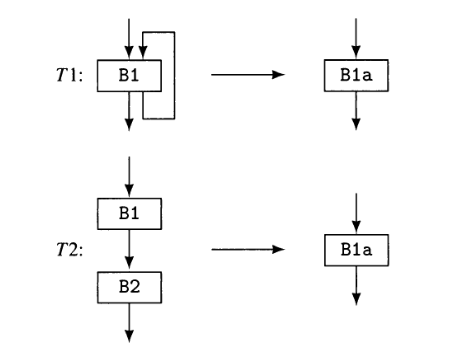
\includegraphics[scale=0.8]{images/t12.png}
\caption{Примеры шаблонов трансформаций для интервального анализа из книги \cite{muchnick1997advanced}}
\label{interval-transformations}
\end{figure}


\subsection{Структурный анализ}
Улучшенной версией
интервального анализа является \emph{структурный анализ}, который отличается тем, что 
определяет
больший набор шаблонов --- областей вершин графа, которые он может идентифицировать. 
Области делятся
на два больших класса: ациклические и циклические. Примеры ациклических шаблонов
приведены на рис.~\ref{acyclic3}.
Отношение доминирования используется в структурном анализе для нахождения
циклических структур (см. рис.~\ref{cyclic}).

\begin{figure}[H]
\centering
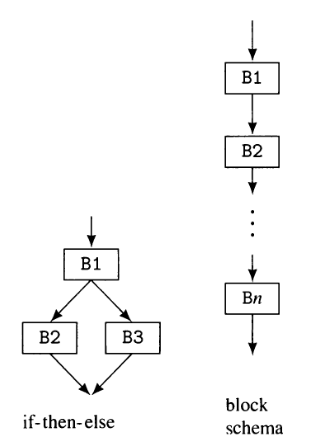
\includegraphics[scale=0.6]{images/acyclic3.png}
\caption{Примеры ациклических регионов для структурного анализа из книги \cite{muchnick1997advanced}}
\label{acyclic3}
\end{figure}


\begin{figure}[H]
\centering
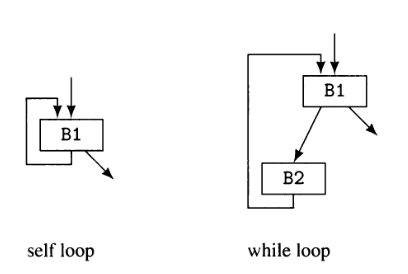
\includegraphics[scale=0.6]{images/cyclic2.png}
\caption{Примеры циклических регионов для структурного анализа из книги \cite{muchnick1997advanced}}
\label{cyclic}
\end{figure}

\subsection{Генерация кода}
Результатом применения интервального и структурного анализов является \emph{дерево управляющих структур}, 
родительские узлы которого представляют собой распознанные шаблоны, а листья --- 
исходные вершины графа. Опишем предполагаемый 
рекурсивный процесс генерации кода, который начинается с корня дерева.
Если текущая вершина --- лист, то генерируем эквивалентный текст для текущего 
целевого языка из текста, 
который задавался при создании данного блока диаграммы. 
Иначе --- вершина является абстрактной (задает некоторую управляющую структуру),
поэтому генерируем код для 
этой управляющей структуры, а затем вызываем процесс генерации от дочерних вершин.

\section{Реализация}
В работе был реализован алгоритм структурного анализа \cite{muchnick1997advanced},
поскольку он обнаруживает сложные структуры, которые есть у большинства языков,
поддерживаемых TRIK Studio.
Для этого был создан класс, который инкапсулирует структуры данных и необходимые
функции. Приведем наиболее важные из них:
\begin{itemize}
    \item метод для вычисления доминаторов каждой вершины графа;
    \item функции для определения циклических и ациклических структур;
    \item функция reduce для удаления лишних вершин;
    \item функция replace для удаления лишних рёбер графа и перенаправления
          других рёбер к новой.
\end{itemize}

Затем он был интегрирован в среду TRIK Studio. На рис.~\ref{cyclic} представлена 
UML-диаграмма классов, которые связаны с генерацией кода.

\begin{figure}[H]
\centering
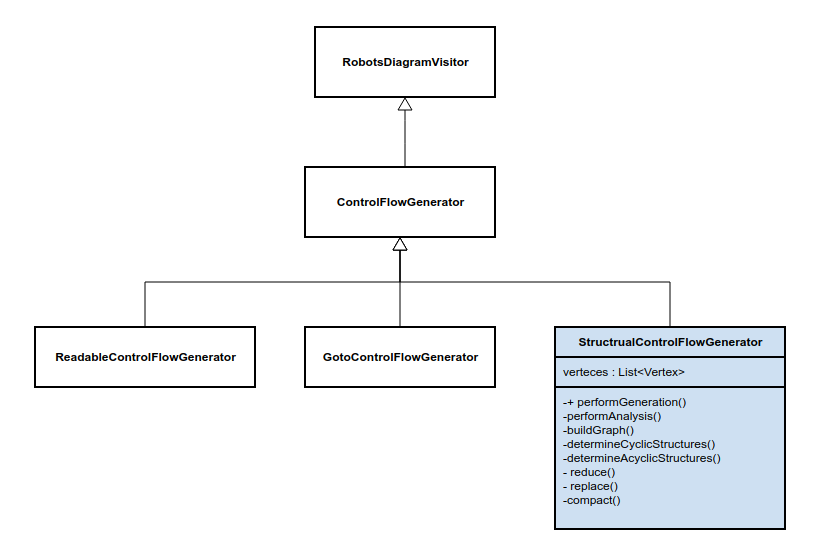
\includegraphics[scale=0.6]{images/uml3.png}
\caption{UML-диаграмма классов, связанных с кодогенерацией в TRIK Studio}
\end{figure}

Светло-синим цветом фона выделен новый класс.
Стоит заметить, что метод replace из книги \cite{muchnick1997advanced}
подвергся лёгкой модификации, поскольку в изначальной
реализации удалялись лишние ребра, которые несли важную информацию.

% У заключения нет номера главы
\section*{Текущие результаты}
Алгоритм был апробирован на реальных диаграммах для роботов. Удалось структурировать
ранее не структурируемую диаграмму (см. рис.~\ref{diagram}).

\begin{figure}[H]
\centering
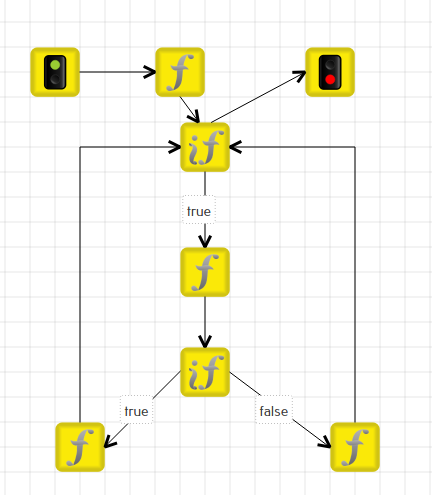
\includegraphics[scale=0.6]{images/diagram1.png}
\caption{Диаграмма управления робота TRIK}
\label{diagram}
\end{figure}

Опишем работу алгоритма детально:
\begin{enumerate}
    \item блоки \textbf{If}, \textbf{function}, \textbf{function}
          образуют абстрактный блок \textbf{IfThenElse} 
          (рис.~\ref{fig:A} --- рис.~\ref{fig:B});
    \item блоки \textbf{If}, \textbf{function}, \textbf{IfThenElse} 
          образуют блок \textbf{Block}
          (рис.~\ref{fig:B} --- рис.~\ref{fig:C});
    \item блок \textbf{Block} идентифицируется как \textbf{SelfLoop}
          (рис.~\ref{fig:C} --- рис.~\ref{fig:D});
    \item оставшиеся блоки распознаются как \textbf{Block}
          (рис.~\ref{fig:D} --- рис.~\ref{fig:E}).
\end{enumerate}


\begin{figure}
    \centering
    \begin{subfigure}[b]{0.4\textwidth}
        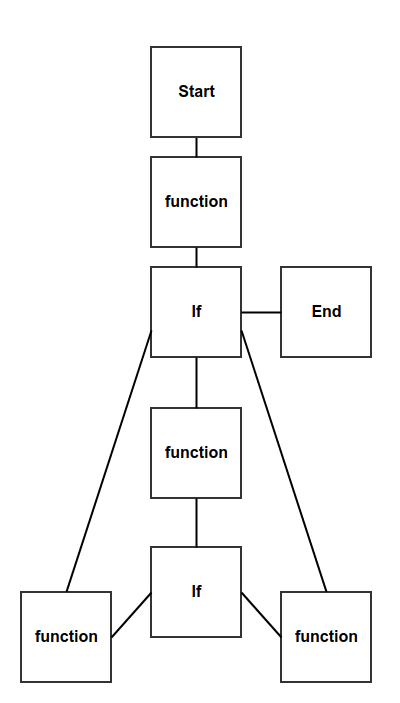
\includegraphics[width=\textwidth]{images/blockScheme1.png}
        \caption{A}
        \label{fig:A}
    \end{subfigure}
    ~ %add desired spacing between images, e. g. ~, \quad, \qquad, \hfill etc. 
      %(or a blank line to force the subfigure onto a new line)
    \begin{subfigure}[b]{0.4\textwidth}
        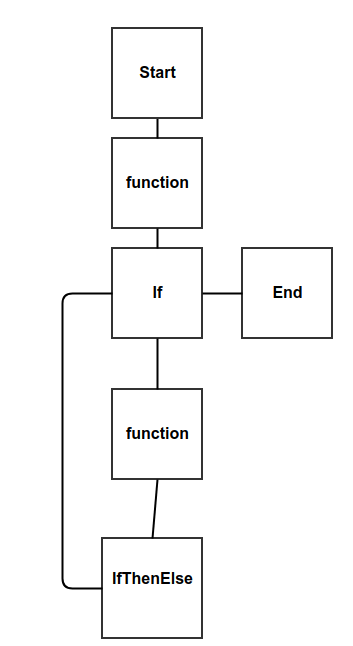
\includegraphics[width=\textwidth]{images/blockScheme2.png}
        \caption{B}
        \label{fig:B}
    \end{subfigure}
    ~ %add desired spacing between images, e. g. ~, \quad, \qquad, \hfill etc. 
    %(or a blank line to force the subfigure onto a new line)
    \begin{subfigure}[b]{0.4\textwidth}
        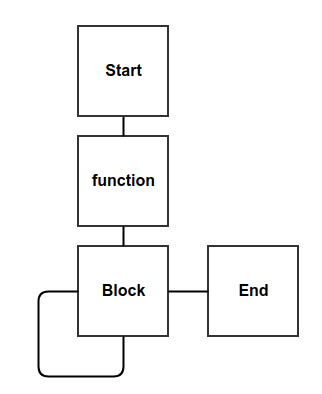
\includegraphics[width=\textwidth]{images/blockScheme3.png}
        \caption{C}
        \label{fig:C}
    \end{subfigure}
    \caption{Преобразование графа потока управления}
\end{figure}

\begin{figure}
    \centering
    \begin{subfigure}[b]{0.4\textwidth}
        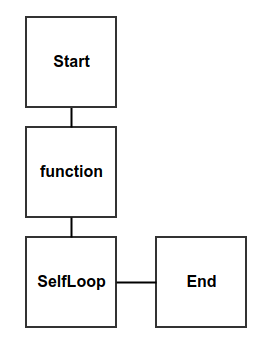
\includegraphics[width=\textwidth]{images/blockScheme4.png}
        \caption{D}
        \label{fig:D}
    \end{subfigure}
    
    \begin{subfigure}[b]{0.4\textwidth}
        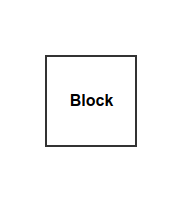
\includegraphics[width=\textwidth]{images/blockScheme5.png}
        \caption{E}
        \label{fig:E}
    \end{subfigure}
    \caption{Преобразование графа потока управления}
\end{figure}


В дальнейшем планируется интегрировать генерацию кода по деревьям управляющих
структур в среду TRIK Studio.

\section*{Заключение}
В результате данной курсовой работы были выполнены следующие задачи:
\begin{itemize}
     \item проведен обзор существующих способов анализа графа потока управления;
     \item был реализован базовый алгоритм структурного анализа в среде TRIK Studio,
           в дальнейшем планируется добавить обработку оставшихся шаблонов структур.
\end{itemize}

\setmonofont[Mapping=tex-text]{CMU Typewriter Text}
\bibliographystyle{ugost2008ls}
\bibliography{diploma.bib}
\end{document}
